\documentclass[../../main.tex]{subfiles}


\begin{document}
    

    \section{Previous Results}
    \section{Event Selection}
    The analysis started using the same procedure used in the NA48/2 \cite{2015178}
    \begin{itemize}
        \item Require either the Control Trigger (sometimes described as Minimum Bias Trigger), Multi Track (MT) or Electron Multi Track (eMT) which are described in Chapter \ref{sec:na62}
        \item A vertex was selected if the total momentum was below $78/,GeV$, a total positive charge of 1, a $\chi^{2}$ less than 40 and a vertex position between 105\, and 180\,m.
        \item The tracks associated to the vertex are selected if they are in acceptance of all four Straw spectrometer chambers and the CHOD. The track momentum must be greater than $5\,GeV$ and less than $60\,GeV$ with a $\Chi^+$ of less than 30. The tracks must traverse within 20\,cm of each other.
        \item Require the presence of a three track in the vertex with a selected positive charged pion ($\pi^+$), and a selected electron positron pair ($\pi^{\pm}$). The pion is selected using missing mass between the Kaon momentum which is taken from the average beam momentum and the two positive tracks. 
        If the positive track is within 5 sigma of the $\pi^0$ mass hypothesis then it is selected as a charged pion. If both positive tracks satisfy the condition the event is vetoed. From MC only approximately $0.1/,\%$ of Dalitz decays have both positive tracks satisfying the selection of the charged pion.
        The electron was assigned to the only negative track and the negative track which doesn't pass the charged pion selection was selected as the positron.
        \item A selected photon is also required. The missing momentum of the vertex was calculated with the Kaon momentum and the total vertex momentum and was used to extrapolate a straight line from the vertex position to the z plane of the LKr calorimeter. Within a radius of 15\,cm of the extrapolated position a single cluster
        with a minimum energy of $5\,GeV$ is selected as a photon from the decay. The photon energy has to satisfy the condition of being within $5\,GeV$ of the calculated missing vertex momentum.
        \item An elliptical cut is used to reduce background that would overwise pass the selection. The reconstructed mass of the electron, positron and photon is compared against the reconstructed mass of the electron, positron, photon and charged pion.
    \end{itemize}
    %%% Plot of the 5 sigma pion selection
    The cut on the reconstructed missing mass of the kaon, charge pion system was calculated using the Dalitz MC sample and is shown in Figure \ref{fig:kaonpion}. The sigma is taken from the fitted guassian on the plot and calculated as, 
    \begin{equation}
        \sigma = 3.984 \pm 0.007
    \end{equation} 
    \begin{figure}[H]
        \centering 
        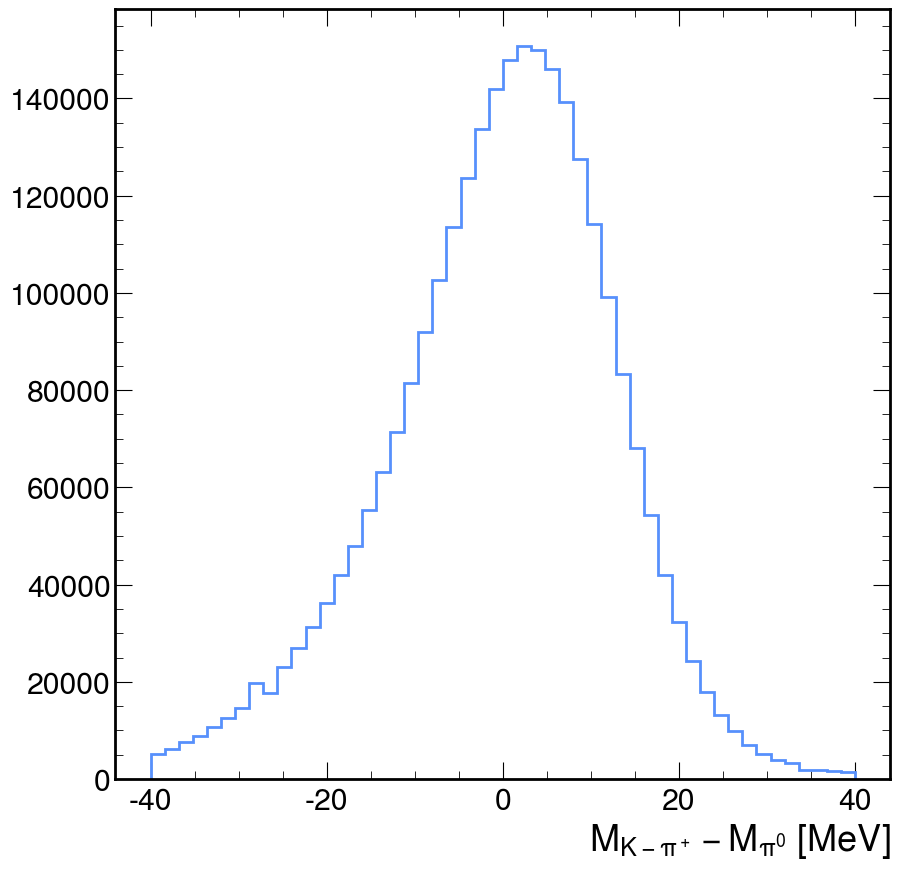
\includegraphics[width=\textwidth]{plots/kaonpion.png}
        \linespread{1.0}
        \caption{Reconstructed missing mass of Kaon and charged pion compared to the known neutral pion mass}
        \label{fig:kaonpion}
    \end{figure}
    The elliptical cut on the final reconstructed masses was defined using the Dalitz MC sample to collect the maximum amount of events passing the selection while making the cut a tight as possible. The simgas for the reconstructed masses $M_{ee \gamma}$ and $M_{\pi ee \gamma}$ is calculated from fitting the distributions shown in Figure \ref{fig:reconMasses}.
    The calculated sigma for the reconstructed mass $M_{\pi ee \gamma}$ was calculated as
    \begin{equation}
        \sigma_M_{\pi ee \gamma} = 2.47 \pm 0.004
    \end{equation}
    and for $M_{ee \gamma}$, 
    \begin{equation}
        \sigma_M_{ee \gamma} = 1.329 \pm 0.009
    \end{equation} 
    which were used as a origin for the elliptical parameters for the cut.
    \begin{figure}[H]
        \centering
        \subfloat{{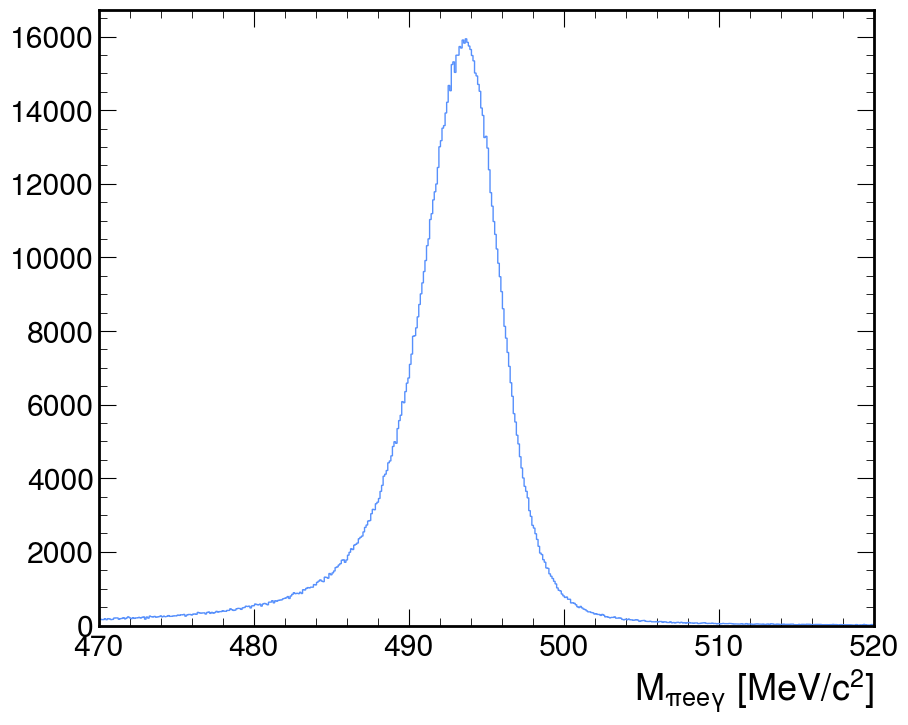
\includegraphics[height=8cm, width=0.5\textwidth]{plots/Mpeeg.png} }}%
        \subfloat{{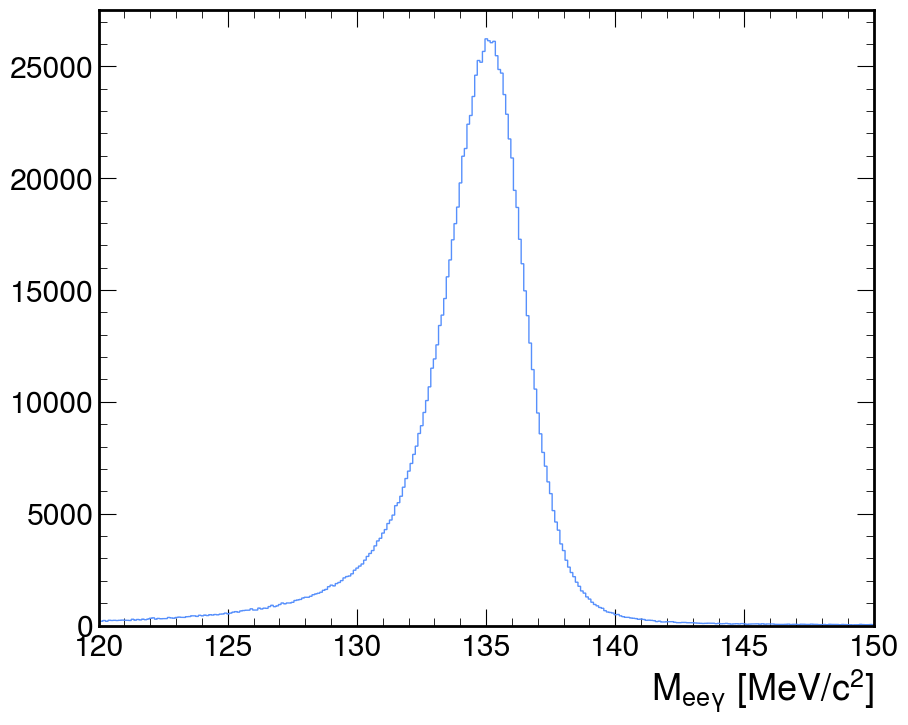
\includegraphics[height=8cm, width=0.5\textwidth]{plots/Meeg.png} }}%
        \linespread{1.0}
        \caption{Reconstructed masses of selected particles, left the total of charged pion, electron, positron and gamma and on right, electron, positron and gamma.}%
        \label{fig:reconMasses}%
    \end{figure}
    The equation used for the elliptical cut in the selection is defined below,
    \begin{equation}
        \frac{((x - x_c)cos(\theta) + (y-y_c)sin(\theta))^2}{a^2} + \frac{((y - y_c)cos(\theta) - (x-x_c)sin(\theta))^2}{a^2} <= 1
    \end{equation}
    where $x_c$ and $y_c$ is the centre of the ellipse in the x and y dimensions. $\theta$ being the rotation of the ellipse, $a$ and $b$ are the length of the semi-major and the semi-minor axis respectively. 
    $x$ and $y$ are the values from the selection and the event is selected if the equation returns a value that is less than or equal to 1. After first starting with the results from Figure \ref{fig:reconMasses} and 
    optimizing for a tight cut with a acceptable number of events passing produced parameters below, 
    \begin{itemize}
        \item $(x_c = 493.37)$: The x-coordinate of the ellipse's center.
        \item $(y_c = 134.89)$: The y-coordinate of the ellipse's center.
        \item $(a = 10.24)$: The semi-major axis of the ellipse ($4 \times \sigma_M_{\pi ee \gamma}$).
        \item $(b = 4.29)$: The semi-minor axis of the ellipse ($3 \times \sigma_M_{ee \gamma}$).
        \item $(\theta = 0.4887)$: The rotation angle of the ellipse in radians.
        \item $((x, y))$: The point being tested for inclusion within the ellipse.
    \end{itemize}
    Which produced an ellipse used in the selection which is shown in \ref{fig:elip}
    \begin{figure}[H]
        \centering 
        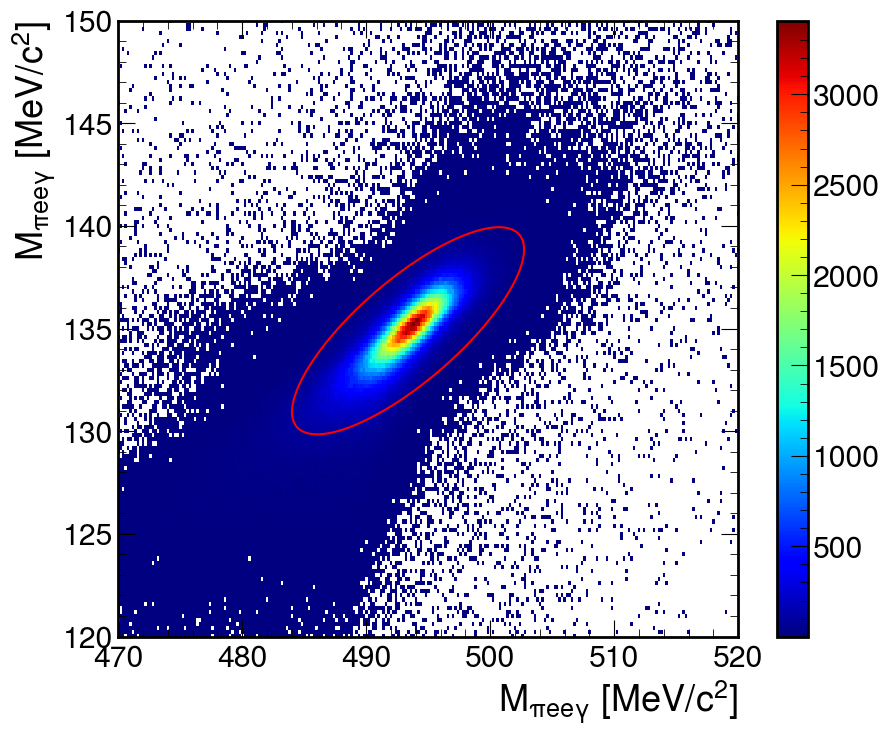
\includegraphics[width=\textwidth]{plots/elip.png}
        \linespread{1.0}
        \caption{Reconstructed missing mass of $M_{\pi ee \gamma}$ compared against $M_{ee \gamma}$ produced from a K2pi Dalitz MC sample, with the defined elliptical cut used in the selection}
        \label{fig:elip}
    \end{figure}
    The acceptance of the Dailtz sample is defined across the reconstructed electron position mass in the range $2m_e < M_ee < m_{\pi^0}$ and is compared against the acceptance of the NA48/2 analysis \cite{2015178} in Figure \ref{fig:accept}.
    Improving the selection using kinematic cuts compared to the calorimeter PID improved the acceptance at high $M_ee$ compared to NA48/2. It was expected that NA48/2 would have an acceptance advantage due to its design as a shorter experiment. If the same analysis procedure was employed using calorimetric PID the acceptance would not be competitive with NA48/2
    \begin{figure}[H]
        \centering 
        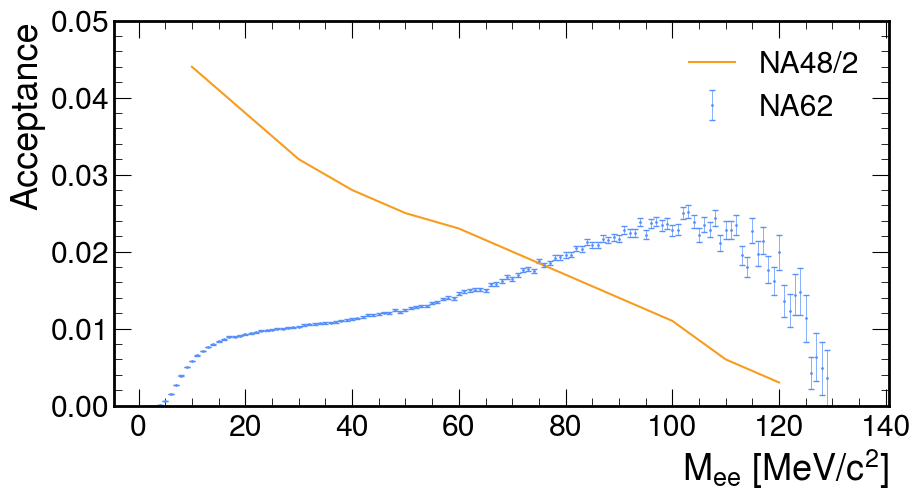
\includegraphics[width=\textwidth]{plots/accept.png}
        \linespread{1.0}
        \caption{Acceptance of the NA62 selection compared against the acceptance produced in the NA48/2 analysis \ref{fig:accept}}
        \label{fig:accept}
    \end{figure}
    \section{Integrated Kaon Flux}

    \ifSubfilesClassLoaded{%
        \bibliographystyle{IEEEtran}
        \bibliography{../../../references.bib}%
    }{} 
\end{document}